\section{Data collection}\label{sec:data-collection}
The data used is the \gls{mnist} database \cite{lecun-mnist-database}, which is a collection of handwritten digits. The data is split into a training set of 60,000 images and a test set of 10,000 images. The images are 28x28 pixels grayscale, and each pixel is the intensity of the pixel represented by a value between 0 and 255, where 0 is black and 255 is white. The images are labeled with the digit they represent creating 10 classes, and the labels are integers between 0 and 9.

\subsection{Data pre-preprocessing}\label{subsec:data-pre-preprocessing}
The data is normalized by dividing each pixel value by 255, so that the values are between 0 and 1. The data is then augmented by rotating the images by 90, 180 and 270 degrees, and flipping the images horizontally and vertically. This results in 10 times as much data as the original \gls{mnist} dataset.\todo{Include all the augmentations we actually use.}

\subsection{Data preprocessing}\label{subsec:data-preprocessing}
The data is then preprocessed by applying linear and non-linear dimensionality reduction techniques. The linear dimensionality reduction techniques are \gls{pca} and \gls{lda}. The non-linear dimensionality reduction techniques are \gls{kpca} and \gls{isomap}. The data is reduced to 2 dimensions, so that it can be visualized.

\section{Model training}\label{sec:model-training}
The \gls{lr} and \gls{cnn} models are then trained on both the original and the preprocessed data. The \gls{lr} model is trained using the \gls{sklearn} library, and the \gls{cnn} model is trained using the Keras library.

\subsection{Evaluation}\label{subsec:evaluation}
The models are evaluated using k-fold cross validation, and the results are averaged. The evaluation metrics are accuracy, precision, recall, f1-score, speed/run time, and memory usage. The confusion matrix covers the first of these. The speed/run time is measured by timing the training of the models, and the memory usage is measured by using the psutil library.

Lastly the models are evaluated on the test set and the results are compared to the results from the cross validation.\question{Do we want to compare our results to the results of other papers?}

\section{Pipeline}\label{sec:pipeline}

An automation pipeline is created based on the model in Figure~\ref{fig:python-pipeline-model}.


\begin{description}
    \setlength\itemsep{0em}
    \item[dataset] mnist
    \item[pre-preprocessing] normalization, data augmentation
    \item[preprocessing] linear and non linear dimensionality reduction (PCA, LDA, Kernel PCA, and ISOMAP)
    \item[models] logistic regression and CNN
    \item[evaluation] accuracy, precision, recall, f1-score, speed/run time, and memory usage
\end{description}


\begin{figure}[htb!]
    \centering
    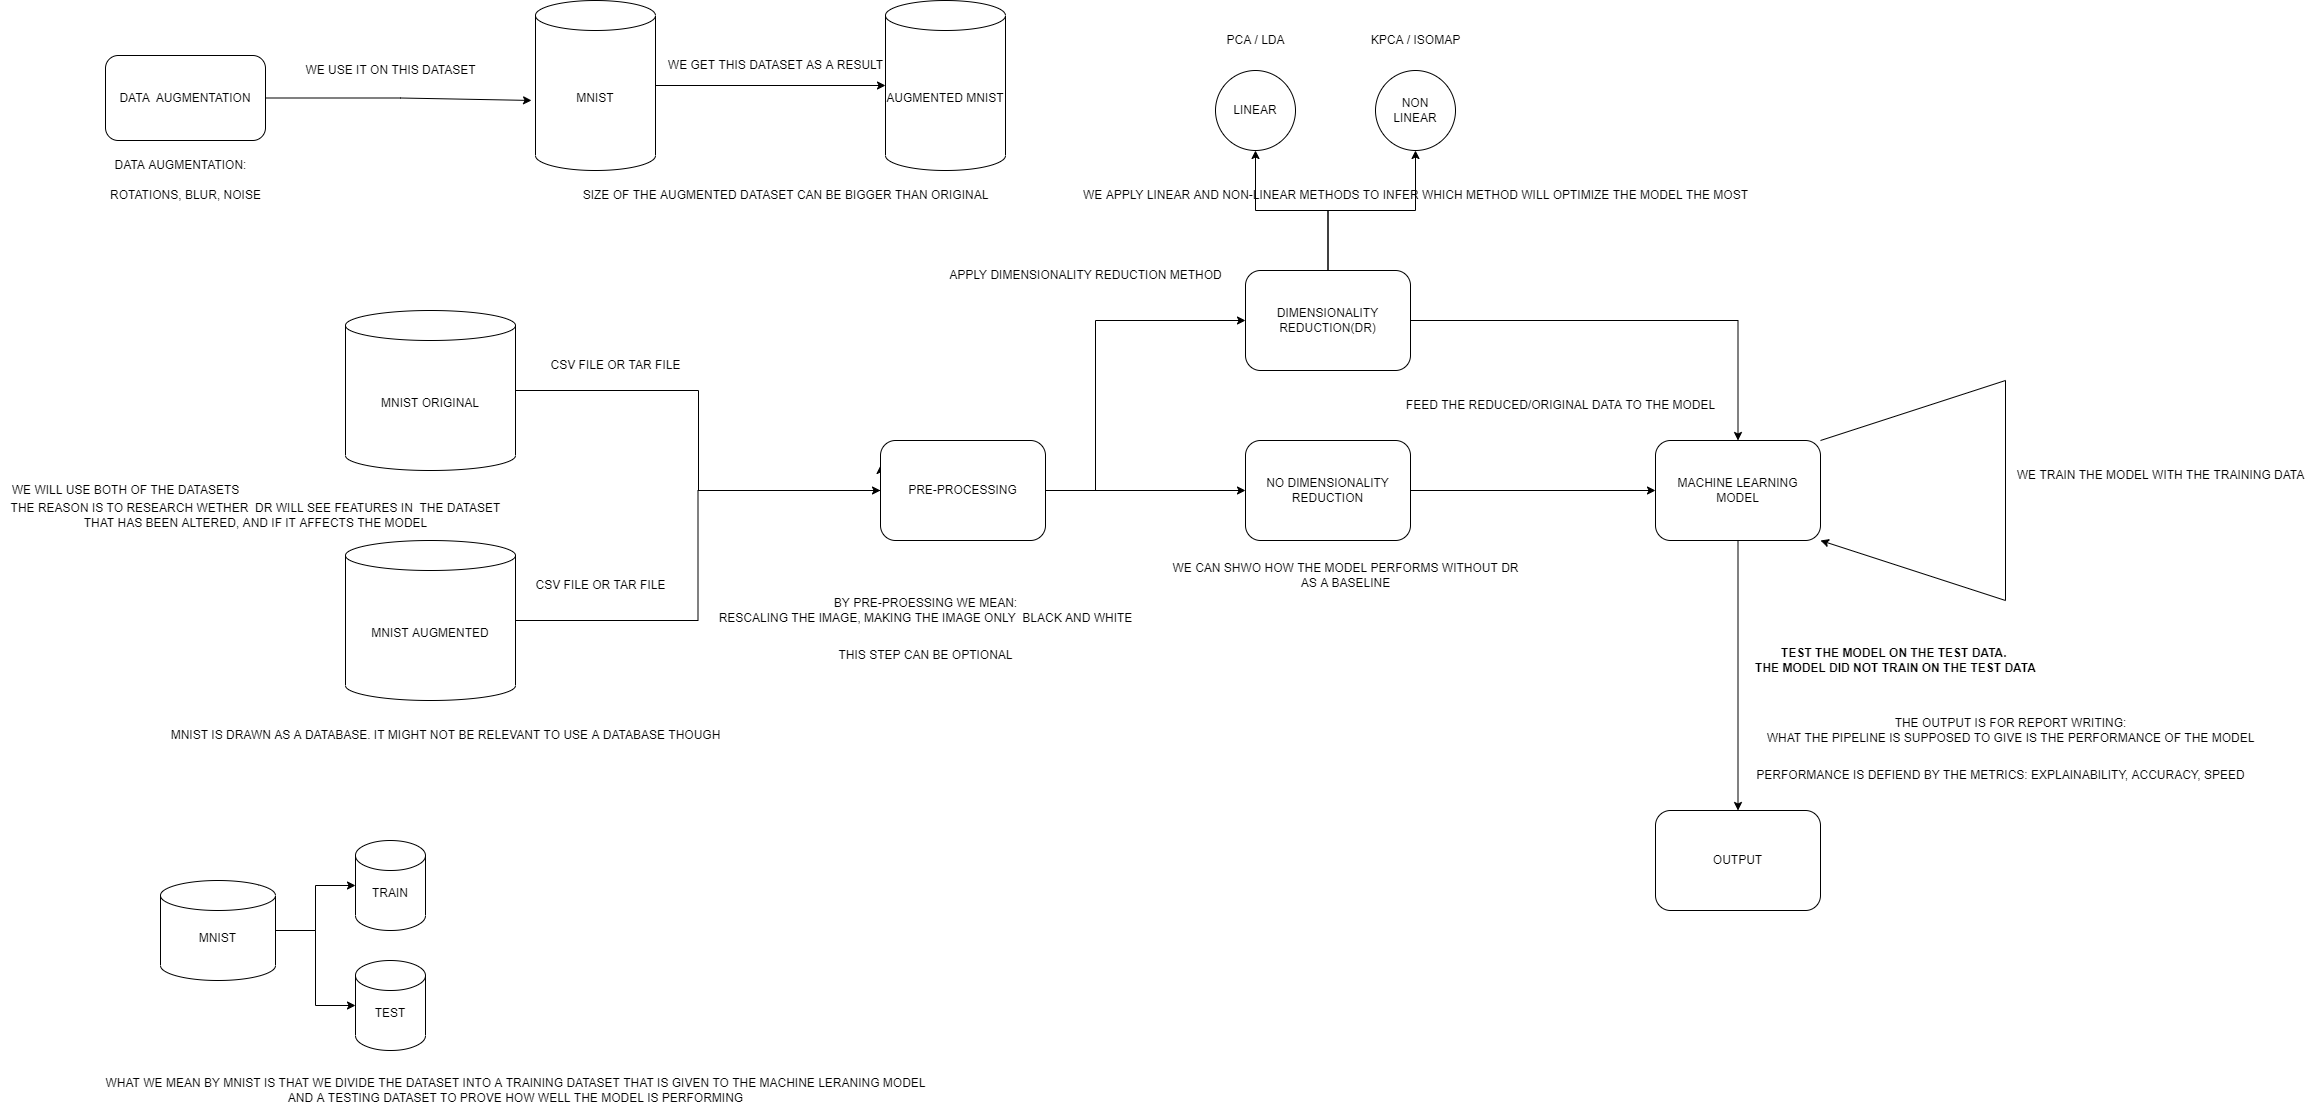
\includegraphics[width=\textwidth]{figures/pipeline-draft.png}
    \caption{Python project pipeline model.}
    \label{fig:python-pipeline-model}
\end{figure}


\urgent[inline]{write about the pipeline, and update the pipeline to include the cross validation.}
